\documentclass[11pt]{article}
\usepackage{graphicx, fullpage}
\usepackage{listings, subcaption}
\graphicspath{{images/}}
\usepackage[utf8]{inputenc}

\begin{document}
\title{Schrödinger Equation Visualized}
\author{Andrew Koller}
\maketitle

\section*{Abstract}
Quantum mechanics courses often introduce the subject in a typical rigorous mathematical style. This paper and subsequent work aims to aid the student or hobbyist in visualizing the solutions to the Schrödinger equation. These visualizations further facilitate an understanding of an already bizarre physical phenomenon. We will examine common quantum systems such as the particle in a box problem and different energy states of the hydrogen atom and animate their behavior when necessary. 

\section{Introduction}
The quantum world is presented as a bizarre otherworldly phenomenon with seemingly infinite complexities. While both assumptions are true, it is not something to be intimidated by. Rather, a picture (visualization) says a thousand words and Erwin Schrödinger ushered in a paradigm shift in physics, the likes of which the world has never seen.

The technology used to visualize this phenomenon is \textit{Python} with its science libraries, \textit{scipy} and \textit{numpy}, and a popular data visualization API called \textit{MayaVi}. Each system requires a fine tuning of the domains of $x, y,$ and $z$. Some systems require a large $z$ domain, while others tend to be more compactly represented. 

\subsection{History}

In January of 1926, Schrödinger published ``\textit{Quantisierung als Eigenwertproblem}" (Quantization as an Eigenvalue Problem) \cite{modernphysics}. In this paper, Schrödinger presented the famous equation 

\begin{equation}
i\hbar\frac{\partial}{\partial t}\Psi = \hat{H}\Psi.
\end{equation}

\noindent This equation simply states that the relationship between the two sides is valid for every eigenstate $\Psi$ of the Hamiltonian $\hat{H}$. With this newly discovered derivation, Schrödinger was able to prove that the solutions to the equation had the same results as previously accepted data for the hydrogen atom. These previously accepted results has its roots in Bohr's model of hydrogen. 

\begin{figure}[h]
	\centering
	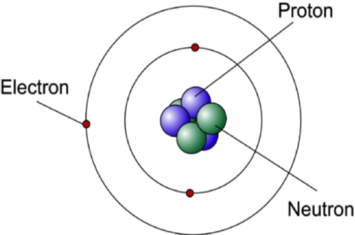
\includegraphics[width = .4\textwidth]{bohrs}
	\caption{Bohr's Model of Hydrogen} 
\end{figure}

\noindent Bohr hypothesized that each electron orbited around the nucleus like planets orbit around each other and their stars \cite{modernphysics}. While this turned out to be inaccurate overall, it was accurate only for the hydrogen atom. Bohr unfortunately did not know because the idea of a quantum system was not relevant at the time. As is with all science, his orbital theory was scrapped when modern quantum mechanics was born.

Schrödinger successfully derived an equation that allows us to understand energy eigenstates of a quantum system. This means that the solutions represent a quantum particle in real and imaginary space. When the scale of measurement enters the scale of atomic, our macroscopic understand of matter collapses into a concept known as wave-particle duality. Each quantum particle can be thought of as a physical piece of matter, but it is also represented as a wave \cite{modernphysics}. 

\section{Particle in a Box}
One of the most popular quantum mechanical systems is the ``Particle in a Box" and will be the first system visualized. The ``box" is a cube where its walls are defined as infinite potential energy. This means that the particle is trapped within this box and cannot escape. The box essentially is an infinite potential well and can be thought of as a stone at the bottom of a hill; without any external force acting on the stone, it will never be able to climb the hill and overcome the gravitational potential of the hill. Given the Schrödinger equation, we expand its components:

\begin{equation}
\frac{-\hbar^2}{2m}\frac{\partial^2}{\partial x^2}\psi + U(x)\psi = E\psi.
\end{equation}

This is known as the one-dimensional time independent equation where $U(x)$ is the potential, $E$ is the energy, and $\psi$ is the wave function. This can be thought of as a statement of conservation of energy within a quantum system. The left hand of the equation is the kinetic plus the potential and the right side is the total energy \cite{modernphysics}. 

\subsection{2-dimensional box}

Because it is not the aim of this paper to work through solutions and derivations of mechanical systems, I'll simply present the solution to a particle in a one-dimensional box. The equation is a second order differential equation, so we expect a sinusoidal wave solution: 

\begin{equation}
\Psi(x, t) = \psi(x)\phi(t) = \sqrt{\frac{2}{L_x}}sin(kx)e^{-i\omega t}
\end{equation}

\noindent where $L_x$ is the length of the potential well (box) and $e^{-i\omega t}$ is the time component. Extending this equation into two dimensions simply adds another $sine$ function and an extra dimension to the box:

\begin{equation}
\Psi(x, y, t) = \sqrt{\frac{4}{L_x L_y}}sin(k_x x)sin(k_y y)e^{-i\omega t}.
\end{equation}

An essential part of this equation are the arguments of the sine functions. Within the solution, $k_x = \frac{n_x\pi}{L_x}$ and $k_y = \frac{n_y\pi}{L_y}$. $n_x$ and $n_y$ are referred to as the \textit{quantum numbers}. These numbers are discrete values, $n = 0, 1, ..., m$, and help define valid solutions to the Schrödinger equation. We begin by defining the domain of values for $x$ and $y$. It is important to recognize and understand these discrete values. Each eigenstate of the quantum system is discrete itself, the quantum numbers help represent these states \cite{modernphysics}.   

\begin{verbatim}
x, y = numpy.mgrid[0:1:.01, 0:1:.01]
\end{verbatim}

\noindent where $x$ and $y$ become a 100x100 mesh. MayaVI's functionality includes a 2-dimensional surf plot:

\begin{verbatim}
s = surf(x, y, f, warp_scale="auto").
\end{verbatim}

This wave, when animated, represents the particle's oscillatory behavior. This should not be mistaken with \textit{where} the particle is.

\begin{figure}[h]
	\centering
	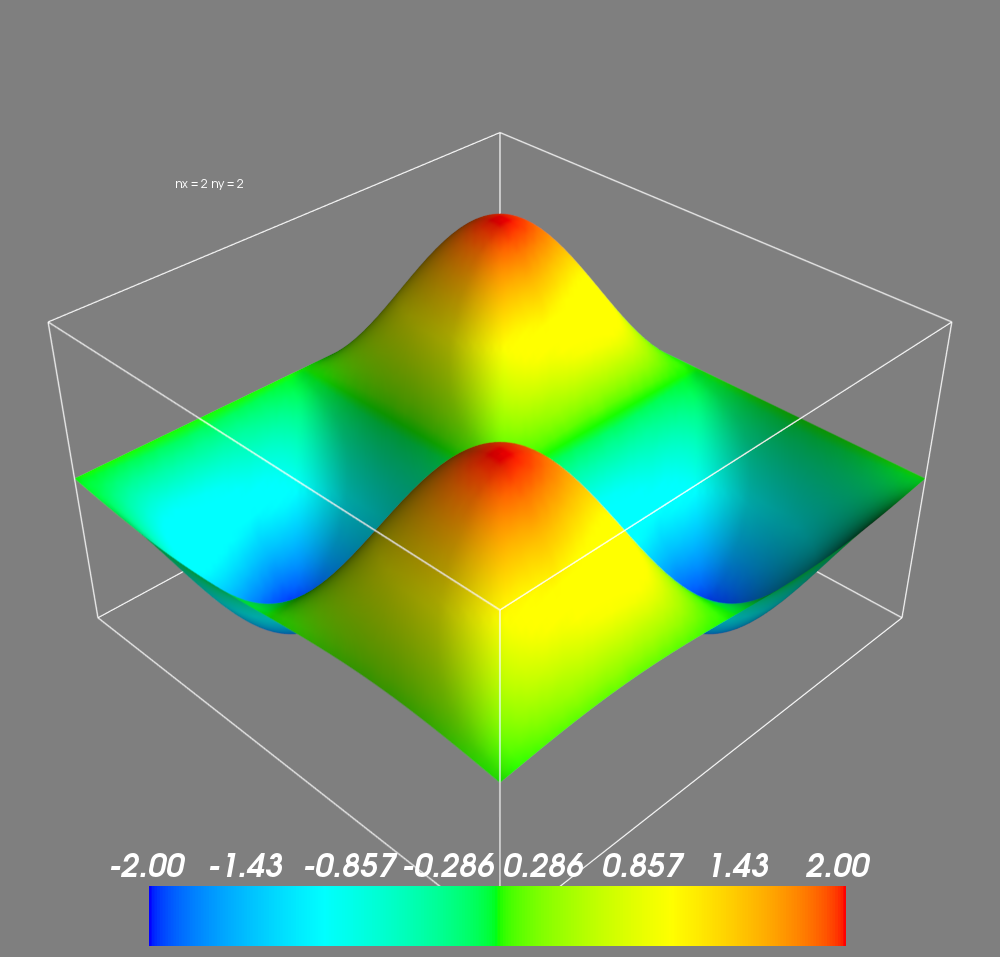
\includegraphics[width = .5\textwidth]{2d22}
	\caption{2D particle in a box where $L_x = 1$, $L_y = 1$, $n_x = 2$, and $n_y = 2$}
\end{figure}

To be able to determine where the particle is, we must square the overall wave function which results in a probability density. During the entire cycle of the wave function, there are positions where the wave function remains at zero. This means the the probability of finding the particle at this location is exactly zero. Figure 3 represents the probability density of this system. If an experiment is being done on this system, a human observer will need to look for the particle in the high probability peaks. 

\begin{figure}[h]
	\centering
	\caption{2D particle in a box \textbf{probability density} where $L_x = 1$, $L_y = 1$, $n_x = 2$, and $n_y = 2$}
	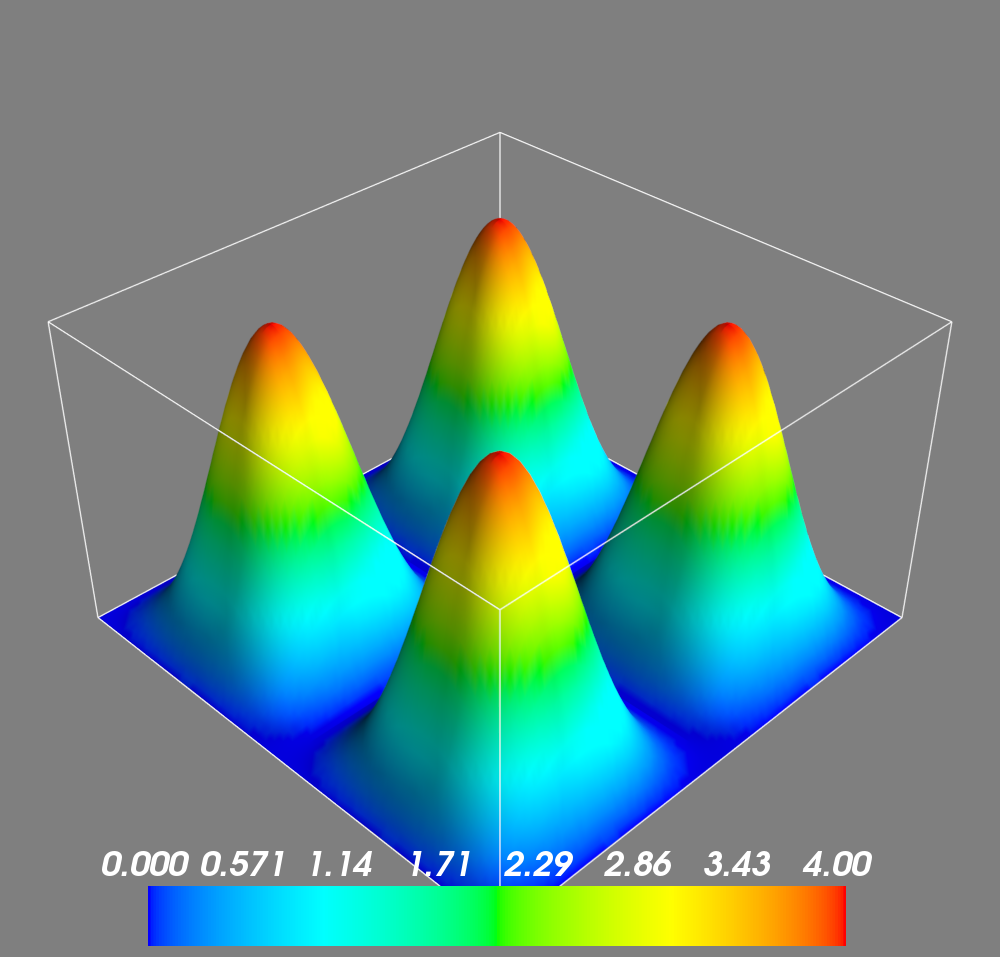
\includegraphics[width = .5\textwidth]{2d22squared}
\end{figure}

\subsection{3-dimensional box}
Extending this problem into three dimensions follows the 2D pattern. Equation (5) doubles the argument within the square root and adds yet another sine function. The 3D box however does not contain simple peaks and valleys. 

\begin{equation}
\Psi(x, y, z, t) = \sqrt{\frac{8}{L_x L_y L_z}}sin(k_x x)sin(k_y y)sin(k_z z)e^{-i\omega t}.
\end{equation}

These systems take the shape of spheres ``hovering" in 3D space. The empty space between each sphere corresponds to areas where the particle will never be found. Each sphere has different layers of contours again representing a more dense probability. Defining the \textit{numpy} mesh in this case requires a $z$ component and extending the box into 3-dimensions also requires a new function call to generate the isosurfaces. 

\begin{verbatim}
x, y = numpy.mgrid[0:1:.01, 0:1:.01, 0:1:.01]
contour3d(x, y, z, f)
\end{verbatim}



\noindent where $f$ is our $\psi$ wave function. Figure 4 displays a sphere representing the particle in the center of the box. The darker red center corresponds to high probability areas, while the lighter blue has a lower probability. A plane oriented on the $y$-axis is included in Figure 5 to help provide a visual of the cross-section of the sphere. The command 
\begin{verbatim}
image_plane_widget(plot, plane_orientation='y_axes', slice_index=10)|
\end{verbatim}


\noindent produces the cross-section plane seen in Figure 5. As the quantum numbers are increased, the density of spheres representing the particle increase. 


\begin{figure}[!tbp]
	\centering
	\begin{minipage}[b]{0.4\textwidth}
		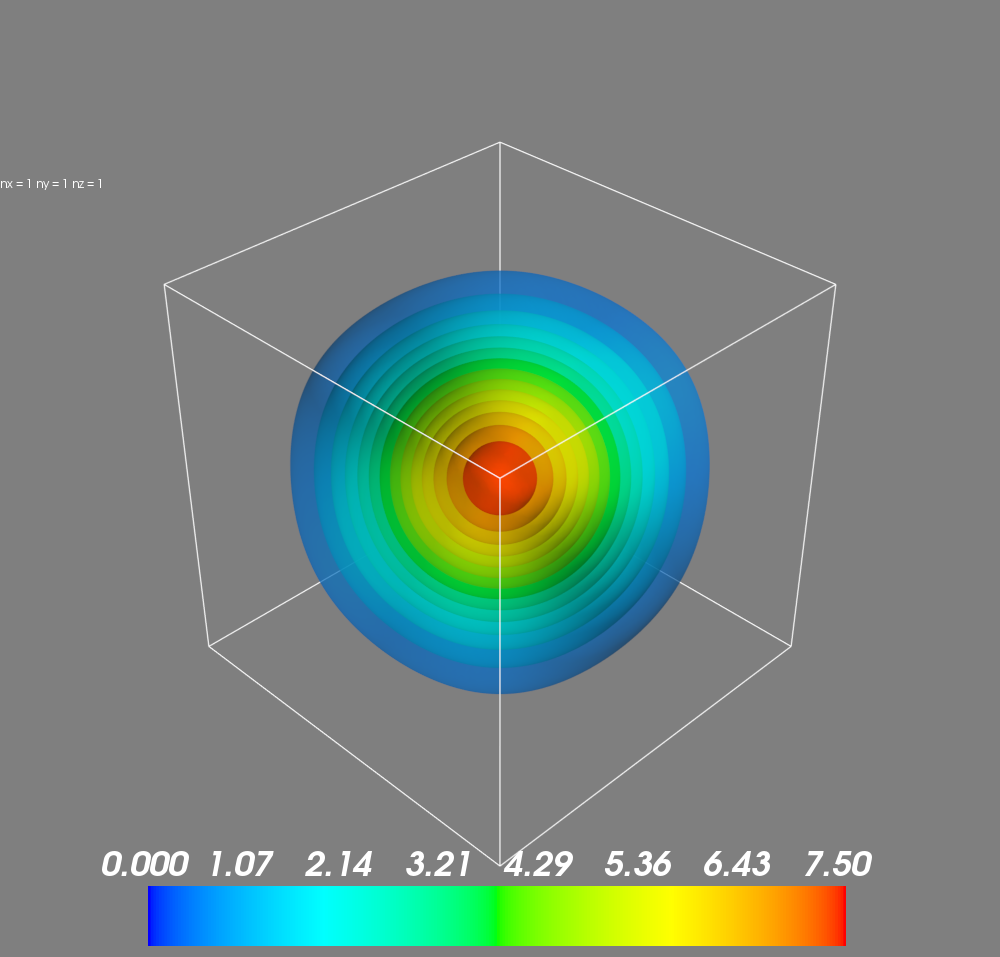
\includegraphics[width=\textwidth]{3d111}
		\caption{3D particle in a box where $L_x, L_y, L_z = 1$, $n_x, n_y, n_z = 1$}
	\end{minipage}
	\hfill
	\begin{minipage}[b]{0.4\textwidth}
		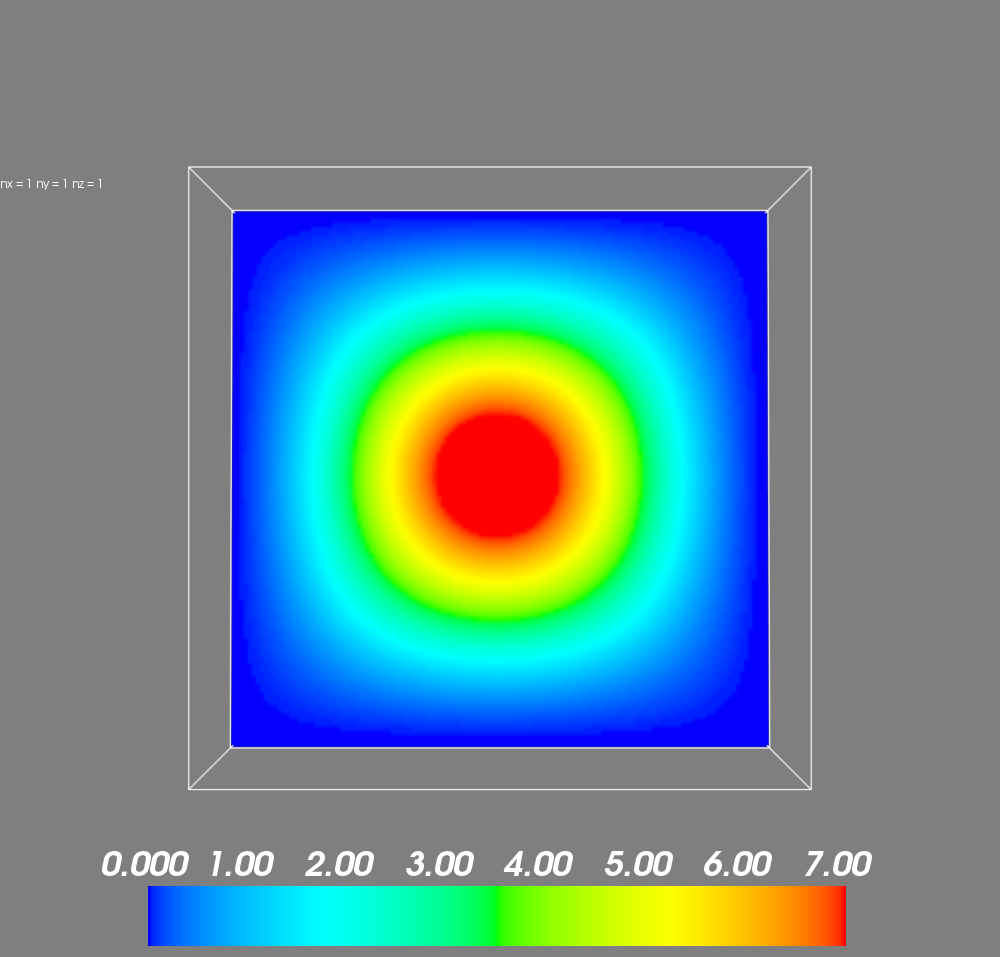
\includegraphics[width=\textwidth]{3d111_cross}
		\caption{3D particle cross-section of Figure 4}
	\end{minipage}
\end{figure}

\begin{figure}[!tbp]
	\centering
	\begin{minipage}[b]{0.4\textwidth}
		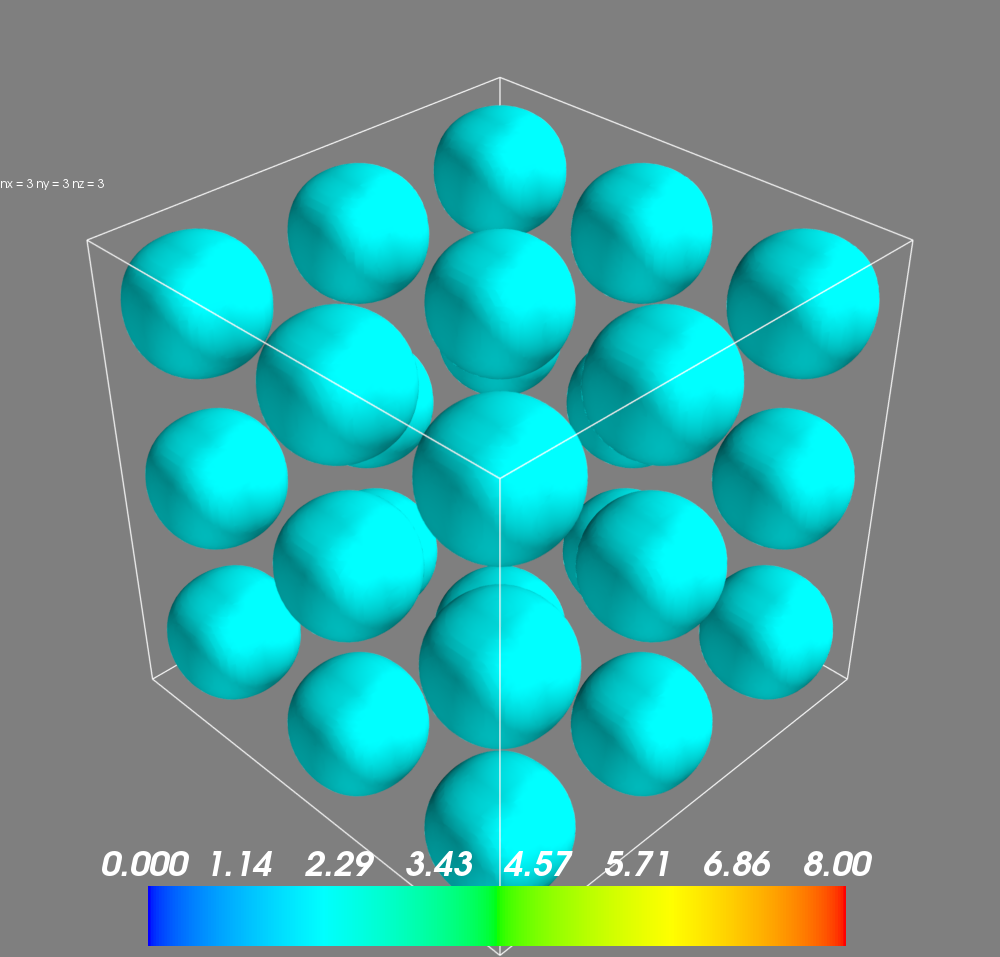
\includegraphics[width=\textwidth]{3d333}
		\caption{3D particle in a box where $L_x, L_y, L_z = 1$, $n_x, n_y, n_z = 3$. Note that when all of the quantum numbers are the same, the system is symmetric about the $x, y,$ and $z$ axes.}
	\end{minipage}
	\hfill
	\begin{minipage}[b]{0.4\textwidth}
		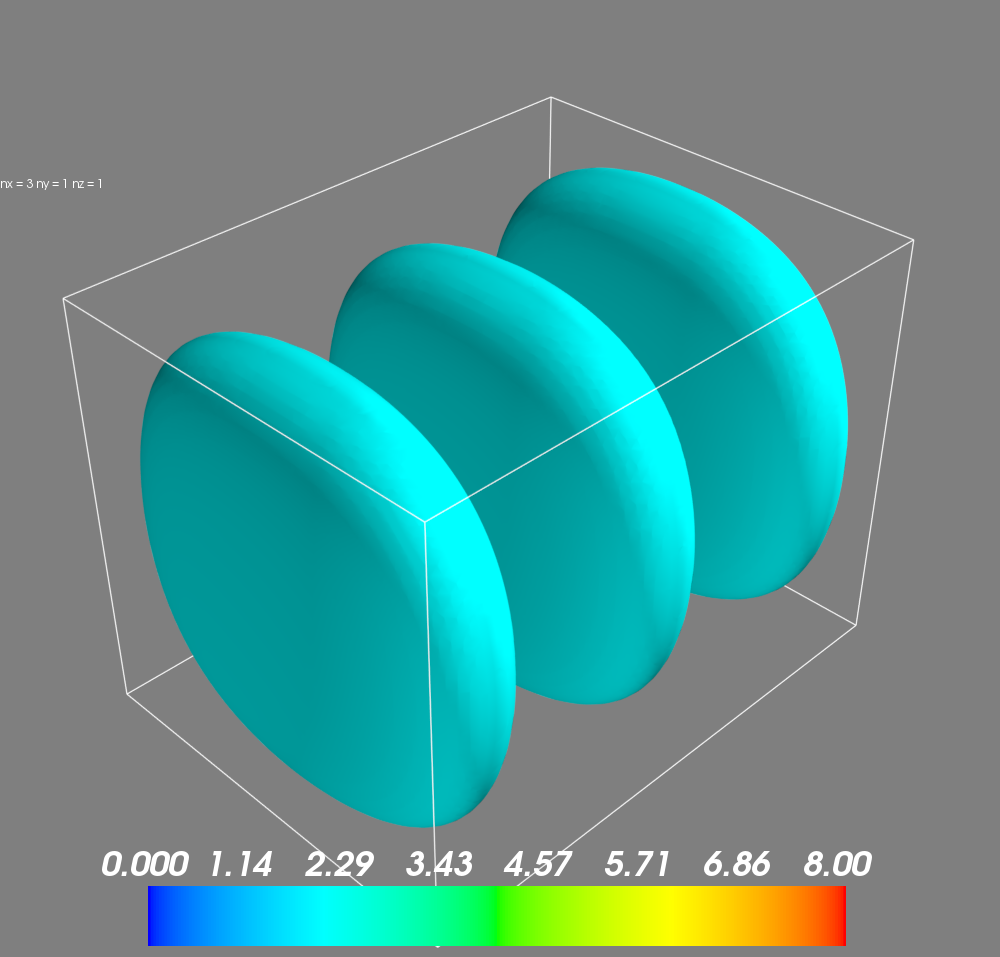
\includegraphics[width=\textwidth]{3d311}
		\caption{3D particle in a box where $L_x, L_y, L_z = 1$, $n_x = 3, n_y = 1, n_z = 1$. Note that when the quantum numbers are not equal to each other, the probability densities become elongated.}
	\end{minipage}
\end{figure}


The particle in a box system provides an excellent framework for understanding basic quantum mechanics. 

\newpage

\section{Hydrogen Atom}
While the particle in a box provides an excellent framework for understanding quantum systems, the meat of the Schrödinger equation comes from representations of the hydrogen atom. We begin by converting the Schrödinger equation into polar coordinates. This yields a polar equation known as the \textit{radial equation}:

\begin{equation}
\psi(r, \theta, \phi) = R(r)P(\theta)F(\phi)
\end{equation}

\noindent where $R$ is the radial part, $P$ is the polar function, and $F$ is the azimuth function \cite{quantum}. Sparing pages of derivation, the full form of the radial wave equation is

\begin{equation}
\psi_{nlm}(r,\theta,\phi) = \sqrt{\frac{\rho}{r}^3 \frac{(n-l-1)!}{2n(n+l)!}}e^{-\rho / 2}\rho^l L^{2l+1}_{n-l-1}(\rho)Y^{m}_{l}(\theta, \phi)
\end{equation}

\noindent where $\rho = 2r / na_0$, $L$ is the Laguerre polynomial, and $Y$ a spherical harmonic function. These are provided in the \textit{scipy} Python library. 

Solutions to this equation are usually represented as flat, one-dimensional probability density plots \cite{quantum}. The goal of this project is to extend these density plots into isosurfaces that model the entire atom. Firstly, we define the variable $r$ as a three dimensional function of $x, y$, and $z$, $\theta$ as the inverse cosine, and $\phi$ as the inverse tangent.

\begin{verbatim}
r = lambda x, y, z: numpy.sqrt(x**2 + y**2 + z**2)
theta = lambda x, y, z: numpy.arccos(z/r(x,y,z))
phi = lambda x, y, z: numpy.arctan(y/x)
\end{verbatim}

\noindent Secondly, equation (7) is defined and divided into separate parts:

\begin{verbatim}
squared = lambda r, theta, phi, n, l, m: abs(entire_func(r, theta, phi, n, l, m))**2.
\end{verbatim}

\noindent Note that we now have three discrete values, $n, l$, and $m$. $n$ is similar to the particle in a box and represents a discrete value for the energy of the system. $l$ and $m$ refer to the azimuthal quantum number (angular momentum) and the magnetic quantum number, respectively \cite{quantum}. 

During the particle in a box exercise, each mesh of $x, y$, and $z$ was kept uniform according to the dimensions of the box. Here however, we must define the range of values according to what quantum numbers are selected. For instance, for $n = 15, l = 4, m = 0$ the grid is defined as 

\begin{verbatim}
numpy.ogrid[-50:50:100,-50:50:100,-140:140:200]
\end{verbatim}

\noindent so that the $z$ values extend far enough to represent the proper solution. Unfortunately, there was no way of knowing which ranges would correspond to certain quantum numbers, so each solution had to be manually altered until it fit within the plane. MayaVI allows for a specification of how many contours are drawn. Allowing for more contours drastically reduces performance but increases the sharpness of the image.

\begin{verbatim}
contour3d(final_func, contours=32, transparent=True, opacity=.7)
\end{verbatim}

\begin{figure}[!tbp]
	\centering
	\begin{minipage}[b]{0.6\textwidth}
		\caption{Hydrogen atom electron shells with $n = 2, l = 1, m = 0$}
		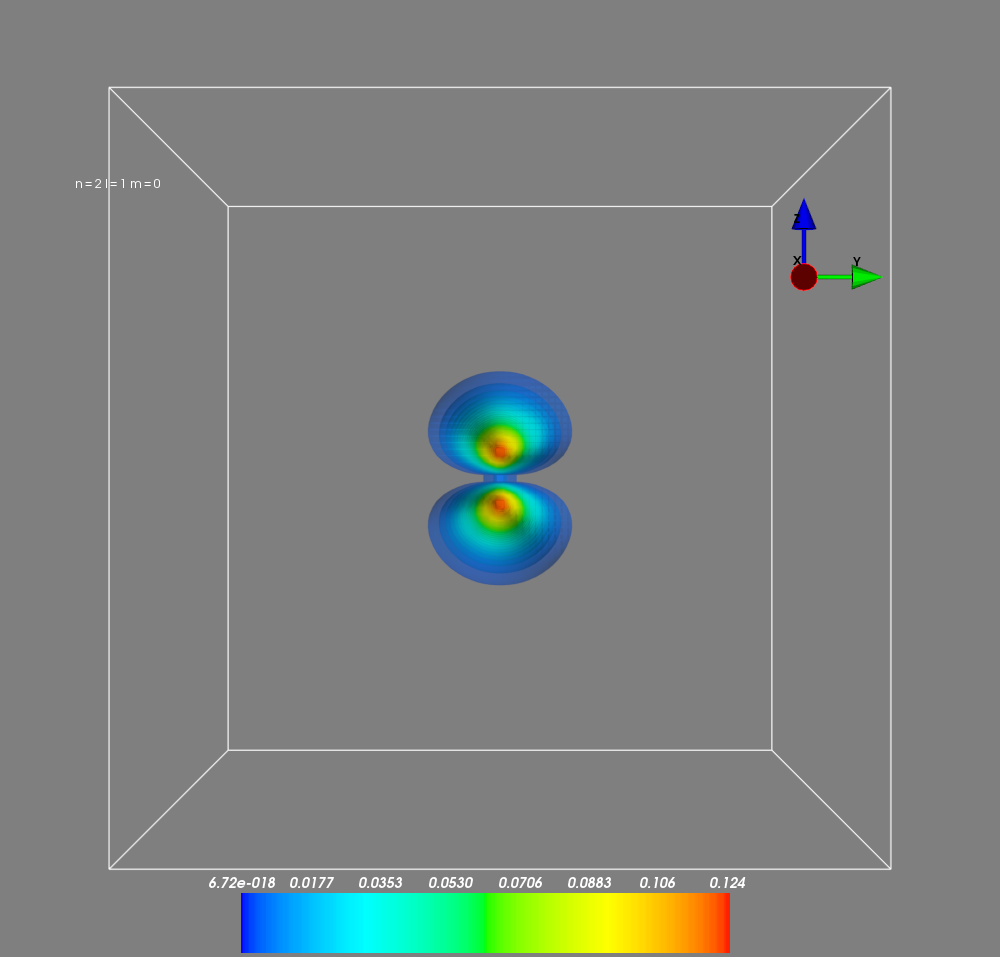
\includegraphics[width=\textwidth]{hydro210}
	\end{minipage}
	\hfill
	\begin{minipage}[b]{0.6\textwidth}
		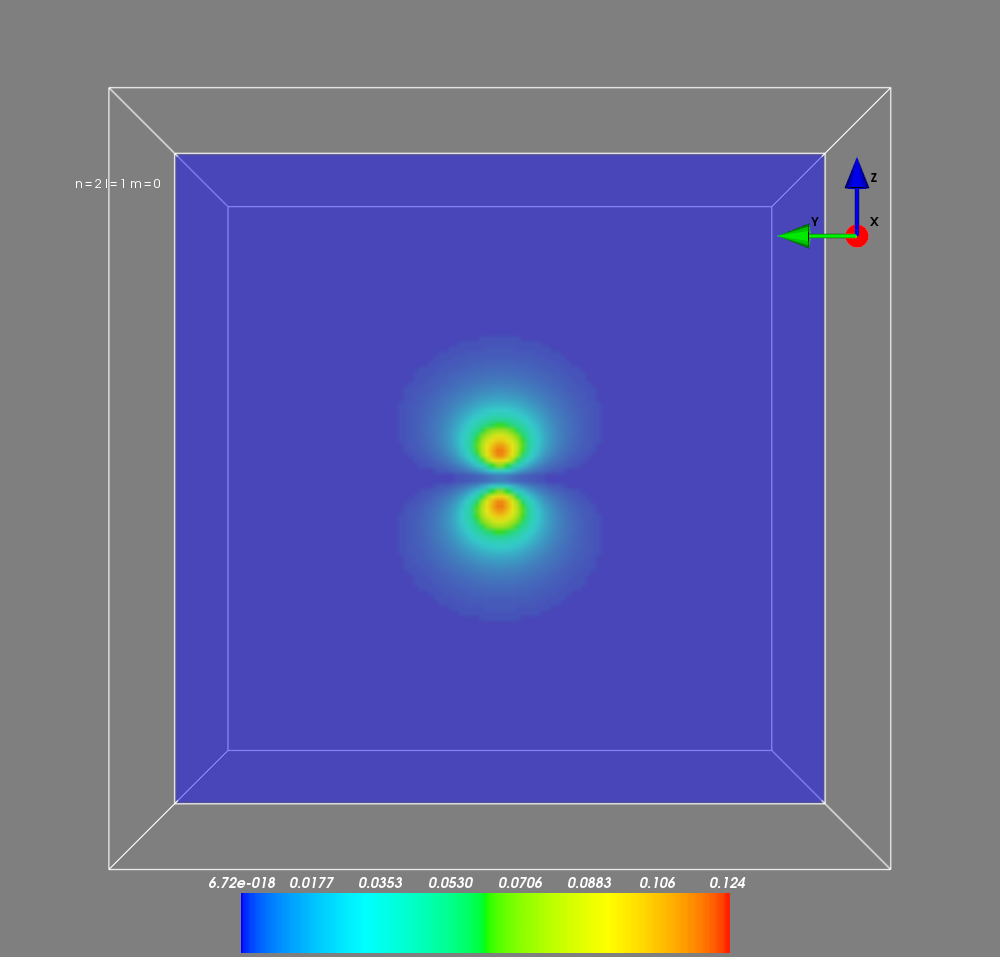
\includegraphics[width=\textwidth]{hydro210_cross}
		\caption{A cross section of Figure 8. This displays a fading probability density from the center to the outer of the shell. The dark blue areas of the plane correspond to zero probability regions, including the divider between the two hemispheres.}
	\end{minipage}
\end{figure}

Figure 8 displays the 3D render of the hydrogen electron shell. The radial equation yields these shells which correspond to the probability density of the electrons orbiting the nucleus. 

\newpage
Each combination of quantum numbers yields increasingly complex systems. Increasing the quantum numbers in effect increases the energy of the system, thus yielding more complex behavior. For instance, with $n = 4, l = 1, m = 0$ the hydrogen atom gains a few more layers to its electron shell. 

\begin{figure}
	\centering
	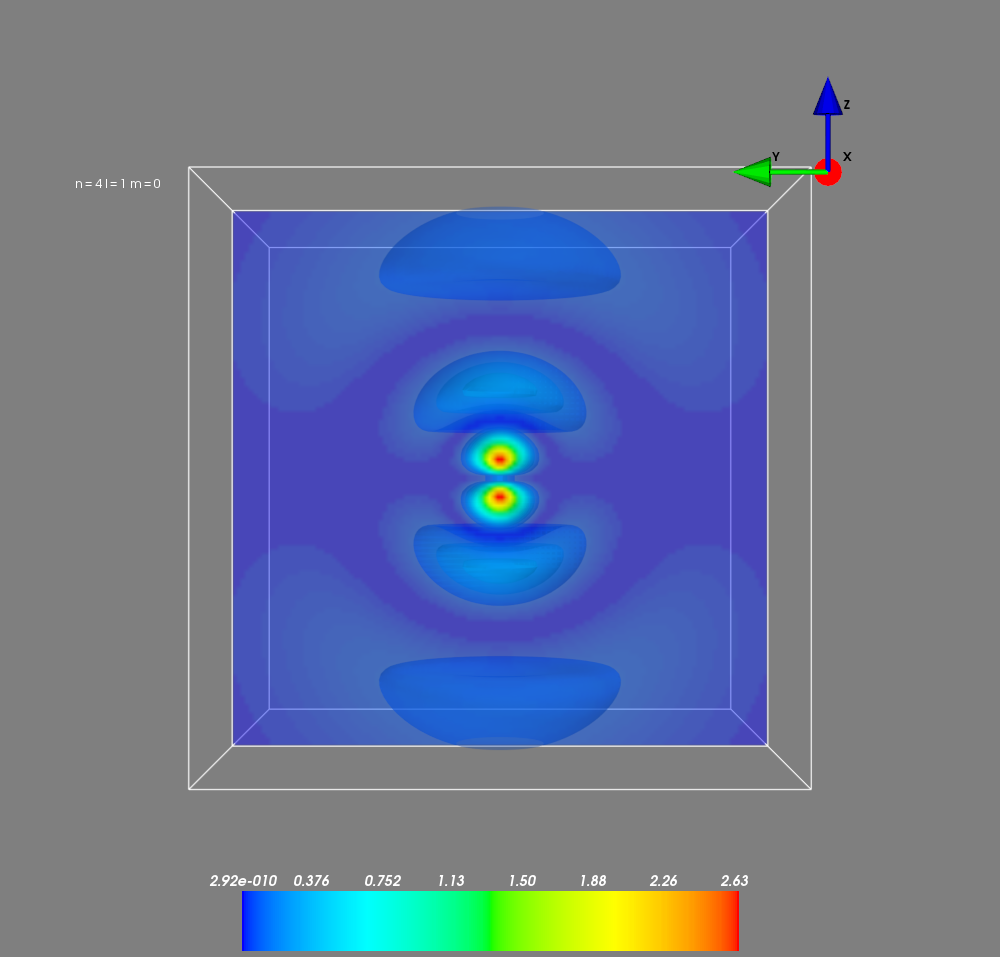
\includegraphics[width = .7\textwidth]{hydro410_cross}
	\caption{Hydrogen atom electron shell with $n = 4, l = 1, m = 0$.}
\end{figure}

\section{Conclusion}
Each section of my project worked out better than I had hoped. Seeing these equations come to life advanced my understanding of the science beyond what I had been taught during my studies. MayaVI, scipy, and numpy provided an excellent framework to process the data and animate it accordingly. One of my original goals of this project was to animate the hydrogen atom. Unfortunately, I did not know that this isn't something typically done. Animation was applied to the particles in a box while I focused my energies on rendering accurate models of the hydrogen atom. 

\newpage

\begin{thebibliography}{9}
\bibitem{modernphysics} 
Randy Harris. 
\textit{Modern Physics Second Edition}. 
University of California, Davis, 2008.

\bibitem{quantum} 
David Griffiths. 
\textit{Introduction to Quantum Mechanics Second Edition}. 
Cambridge University Press, 2016

\bibitem{enthought} 
Enthought 
\textit{Mayavi Documentation}. 
Mayavi version 4.5.0
docs.enthought.com/mayavi/mayavi/index.html


\end{thebibliography}

\end{document}
